\documentclass[12pt, a4paper, simple]{eskdtext}

\usepackage{env}
\usepackage{_sty/gpi_lstlisting}
\usepackage{hyperref}
\usepackage{_sty/gpi_table_of_content}

% Код
\def \gpiDocTypeNum {81}
\def \gpiDocVer {00}
\def \gpiCode {\gpiLetterI\gpieLetterII\gpiLetterIII.\gpiStudentGroupName\gpiStudentGroupNum.\gpiStudentCard.0\gpiDocNum~\gpiDocTypeNum~\gpiDocVer}

% Графа 1 (наименование изделия/документа)
\ESKDcolumnI {\ESKDfontIII
    \gpiTopic \\
    Пояснительная записка
}

% Графа 2 (обозначение документа)
\ESKDsignature {\gpiCode}

% Графа 4 (литералы)
\ESKDcolumnIVfI {\gpiLetterI}
\ESKDcolumnIVfII {\gpieLetterII}
\ESKDcolumnIVfIII {\gpiLetterIII}

% Графа 9 (наименование или различительный индекс предприятия) задает команда
\ESKDcolumnIX {\gpiDepartment}

% Графа 11 (фамилии лиц, подписывающих документ) задают команды
\ESKDcolumnXIfI {\gpiStudentSurname}
\ESKDcolumnXIfII {\gpiTeacherSurname}
\ESKDcolumnXIfV {\gpiTeacherSurname}

\begin{document}
    \begin{ESKDtitlePage}
    \begin{center}
        \gpiMinEdu \\
        \gpiEdu \\
        \gpiKaf \\
    \end{center}

    \vfill

    \begin{center}
        \gpiTopic \\
    \end{center}

    \vfill

    \begin{center}
        \textbf{ПОЯСНИТЕЛЬНАЯ ЗАПИСКА К КУРСОВОЙ РАБОТЕ} \\
        ПО ДИСЦИПЛИНЕ <<\gpiDiscipline>> \\
    \end{center}

    \vfill

    \begin{center}
        \gpiCode \\
        Листов \pageref{LastPage} \\
    \end{center}

    \vfill

    \begin{flushright}
        \begin{minipage}[t]{.49\textwidth}
            \begin{minipage}[t]{.75\textwidth}
                \begin{flushright}
                    Руководитель

                    Выполнил

                    Консультант

                    по ЕСПД
                \end{flushright}
            \end{minipage}
        \end{minipage}
        \begin{minipage}[t]{.49\textwidth}
            \begin{flushright}
                \begin{minipage}[t]{.75\textwidth}
                    \gpiTeacherName~\gpiTeacherSurname

                    \gpiStudentName~\gpiStudentSurname

                    \hspace{0pt}

                    \gpiTeacherName~\gpiTeacherSurname

                \end{minipage}
            \end{flushright}
            
        \end{minipage}
    \end{flushright}

    \vfill

    \begin{center}
        \ESKDtheYear
    \end{center}
\end{ESKDtitlePage}
               % Титульный лист
    % ТЗ
\ESKDthisStyle{empty}
Здесь лист с ТЗ.
\newpage
\ESKDthisStyle{formII}

\tableofcontents                                
\paragraph{Приложение А. Схема программы}
\paragraph{Приложение Б. Текст программы}
\newpage
          % Содержание
    \newpage

\section*{Введение} % Секция без номера
\addcontentsline{toc}{section}{Введение} % Добавить в содержание

В современном мире человеку приходится сталкиваться с огромными массивами однородной информации.
Эту информацию необходимо упорядочить каким-либо образом, обработать однотипными методами
и в результате получить сводные данные или разыскать в массе конкретную информацию.
Этой цели служат базы данных.

База данных — это организованная структура, предназначенная для хранения,
изменения и обработки взаимосвязанной информации, преимущественно больших объемов.

Использование баз данных имеет ряд преимуществ:

\begin{enumerate}
    \item компактность - информация хранится в БД, нет необходимости хранить
    многотомные бумажные картотеки;
    \item скорость - скорость обработки информации (поиск, внесение изменений)
    компьютером намного выше ручной обработки;
    \item низкие трудозатраты - нет необходимости в утомительной ручной работе над данными;
    \item применимость - всегда доступна свежая информация.
\end{enumerate}

На сегодняшний день применение баз данных приобрело весьма важное значение для многих организаций,
которые для упрощения своей работы применяют компьютерные технологии.

Основная цель работы - создание веб приложения, предоставляющего пользователю инструменты для работы
с массивом структурированных данных, содержащем в себе информацию о товарах.

В современном мире программисту приходится сталкиваться с огромным количеством информации,
которую необходимо сохранить.
Хранение информации - это ее запись во вспомогательные запоминающие устройства на различных носителях
для последующего использования.
Хранение является одной из основных операций, осуществляемых над информацией,
и главным способом обеспечения ее доступности в течение определенного промежутка времени.

Информационная система (ИС) - система, предназначенная для хранения, поиска и обработки информации,
и соответствующие организационные ресурсы (человеческие, технические, финансовые и т. д.),
которые обеспечивают и распространяют информацию.

ИС предназначена для своевременного обеспечения надлежащих людей надлежащей информацией,
то есть для удовлетворения конкретных информационных потребностей в рамках определённой
предметной области, при этом результатом функционирования информационных систем является
информационная продукция - документы, информационные массивы, базы данных и информационные услуги.

Первоначально для хранения информации на ЭВМ применялись локальные массивы (или файлы),
при этом для каждой из решаемых функциональных задач создавались собственные файлы исходной
и результатной информации. Это приводило к значительному дублированию данных,
за счёт чего использовалось больше памяти вычислительной машины,
а также усложнялось обновление хранимой информации.

База данных представляет собой определенным образом структурированную совокупность данных,
совместно хранящихся и обрабатывающихся в соответствии с некоторыми правилами.
Как правило, БД моделирует некоторую предметную область или ее фрагмент.
Очень часто в качестве постоянного хранилища информации баз данных выступают файлы.

Немаловажной является и взаимосвязь информации в базе данных: изменение одной строчки
может привести к значительным изменениям других строк.
Работать с данными таким образом гораздо проще и быстрее,
чем если бы изменения касались только одного места в базе данных.

Помимо основной функции - хранения и систематизации огромного количества информации - они
позволяют быстро обрабатывать клиентские запросы и выдавать актуальную информацию.

На сегодняшний день базы данных занимают одно из первых мест для многих организаций,
которые для упрощения своей работы применяют компьютерные технологии.

Результатом разрабатываемой программы должно являться приложение,
позволяющее пользователю взаимодействовать с данными о товарах при помощи пользовательского интерфейса.

\newpage
                   % Введение
    \newpage

\section{ПОСТАНОВКА ЗАДАЧИ}

% = = = = =

\subsection{Перечень функций}

Достижение цели курсовой работы предполагает необходимость создания приложения
для работы с локальной базой данных на тему <<Товары>> с использованием пользовательского
интерфейса и решения следующих конкретных задач:

\begin{enumerate}
    \item добавление товара в базу данных;
    \item вывод товаров из базы данных;
    \item удаление товара из базы данных;
    \item изменение товара в базу данных;
    \item сохранение товаров из базы данных в файл JSON;
    \item сохранение товаров из базы данных в файл CSV;
    \item открытие файла JSON и добавление товаров в базу данных.
\end{enumerate}

% = = = = =

\subsection{Требования пользователей}

Пользовательские требования - описание на естественном языке (плюс поясняющие диаграммы) функций,
выполняемых системой, и ограничений, накладываемых на неё.

Источники: Пользователь

Документ: Пользовательские требования / требования к ПО.

Ответственный: Системный аналитик.

Эти требования должны определять только внешнее поведение системы,
избегая по возможности определения структурных характеристик системы.
Пользовательские требования должны быть написаны естественным языком с использованием
простых таблиц, а также наглядных и понятных диаграмм.

Требования пользователя к информационной системе:

Обязательные:

\begin{enumerate}
    \item должна быть реализована функция ввода данных в информационную систему;
    \item должна работать функция удаления записи из информационной системы.
\end{enumerate}

Желательные:

\begin{enumerate}
    \item информационная система должна выводить отчеты на печать.
\end{enumerate}

% = = = = =

\subsection{Проектирование архитектуры ПО (модули)}

Архитектура программного обеспечения (англ. software architecture) - совокупность
важнейших решений об организации программной системы.

Архитектура включает:

\begin{itemize}
    \item выбор структурных элементов и их интерфейсов, с помощью которых составлена система,
    а также их поведения в рамках сотрудничества структурных элементов
    \item соединение выбранных элементов структуры и поведения во всё более крупные системы
    \item архитектурный стиль, который направляет всю организацию - все элементы, их интерфейсы,
    их сотрудничество и их соединение.
\end{itemize}

Документирование архитектуры программного обеспечения (ПО) упрощает процесс коммуникации
между разработчиками, позволяет зафиксировать принятые проектные решения
и предоставить информацию о них эксплуатационному персоналу системы,
повторно использовать компоненты и шаблоны проекта в других.

Архитектурный вид состоит из 2 компонентов:

\begin{enumerate}
    \item [1.] Элементы
    \item [2.] Отношения между элементами
\end{enumerate}

Архитектурные виды можно поделить на 3 основных типа:

\begin{itemize}
    \item [1.] Модульные виды (англ. module views) - показывают систему как структуру
    из различных программных блоков.
    \item [2.] Компоненты-и-коннекторы (англ. component-and-connector views) - показывают
    систему как структуру из параллельно запущенных элементов (компонентов)
    и способов их взаимодействия (коннекторов).
    \item [3.] Размещение (англ. allocation views) - показывает размещение
    элементов системы во внешних средах.
\end{itemize}

Примеры модульных видов:

Декомпозиция (англ. decomposition view) - состоит из модулей в контексте
отношения <<является подмодулем>>.

Использование (англ. uses view) - состоит из модулей в контексте
отношения <<использует>> (т.е. один модуль использует сервисы другого модуля).

Вид уровней (англ. layered view) - показывает структуру,
в которой связанные по функциональности модули объединены в группы (уровни).

Вид классов/обобщений (англ. class/generalization view) - состоит из классов,
связанные через отношения <<наследуется от>> и <<является экземпляром>>.

\subsubsection*{Иерархия модулей и подмодулей разрабатываемой программы для frontend}

Информационная система включает в себя следующие модули на frontend:

\begin{itemize}
    \item модуль не найденной страницы
    \item модуль авторизации
    \item модуль выхода
    \item модуль меню
    \begin{itemize}
        \item модуль, реализующий добавление новых записей в базу данных;
        \item модуль организации локальной базы данных с выводом информации о товарах;
        \begin{itemize}
            \item модуль удаления записи из локальной базы данных;
        \end{itemize}
        \item модуль, осуществляющий изменение записи;
        \item модуль, осуществляющий сохранение данных в JSON;
        \item модуль, осуществляющий сохранение данных в CSV;
        \item модуль, осуществляющий открытие файла JSON.
    \end{itemize}
\end{itemize}

Схема frontend модулей изображена на
\textbf{рис. \ref{fig:gpi_frontend_modules} (стр. \pageref{fig:gpi_frontend_modules})}.

\begin{figure}[!htp]
    \centering
    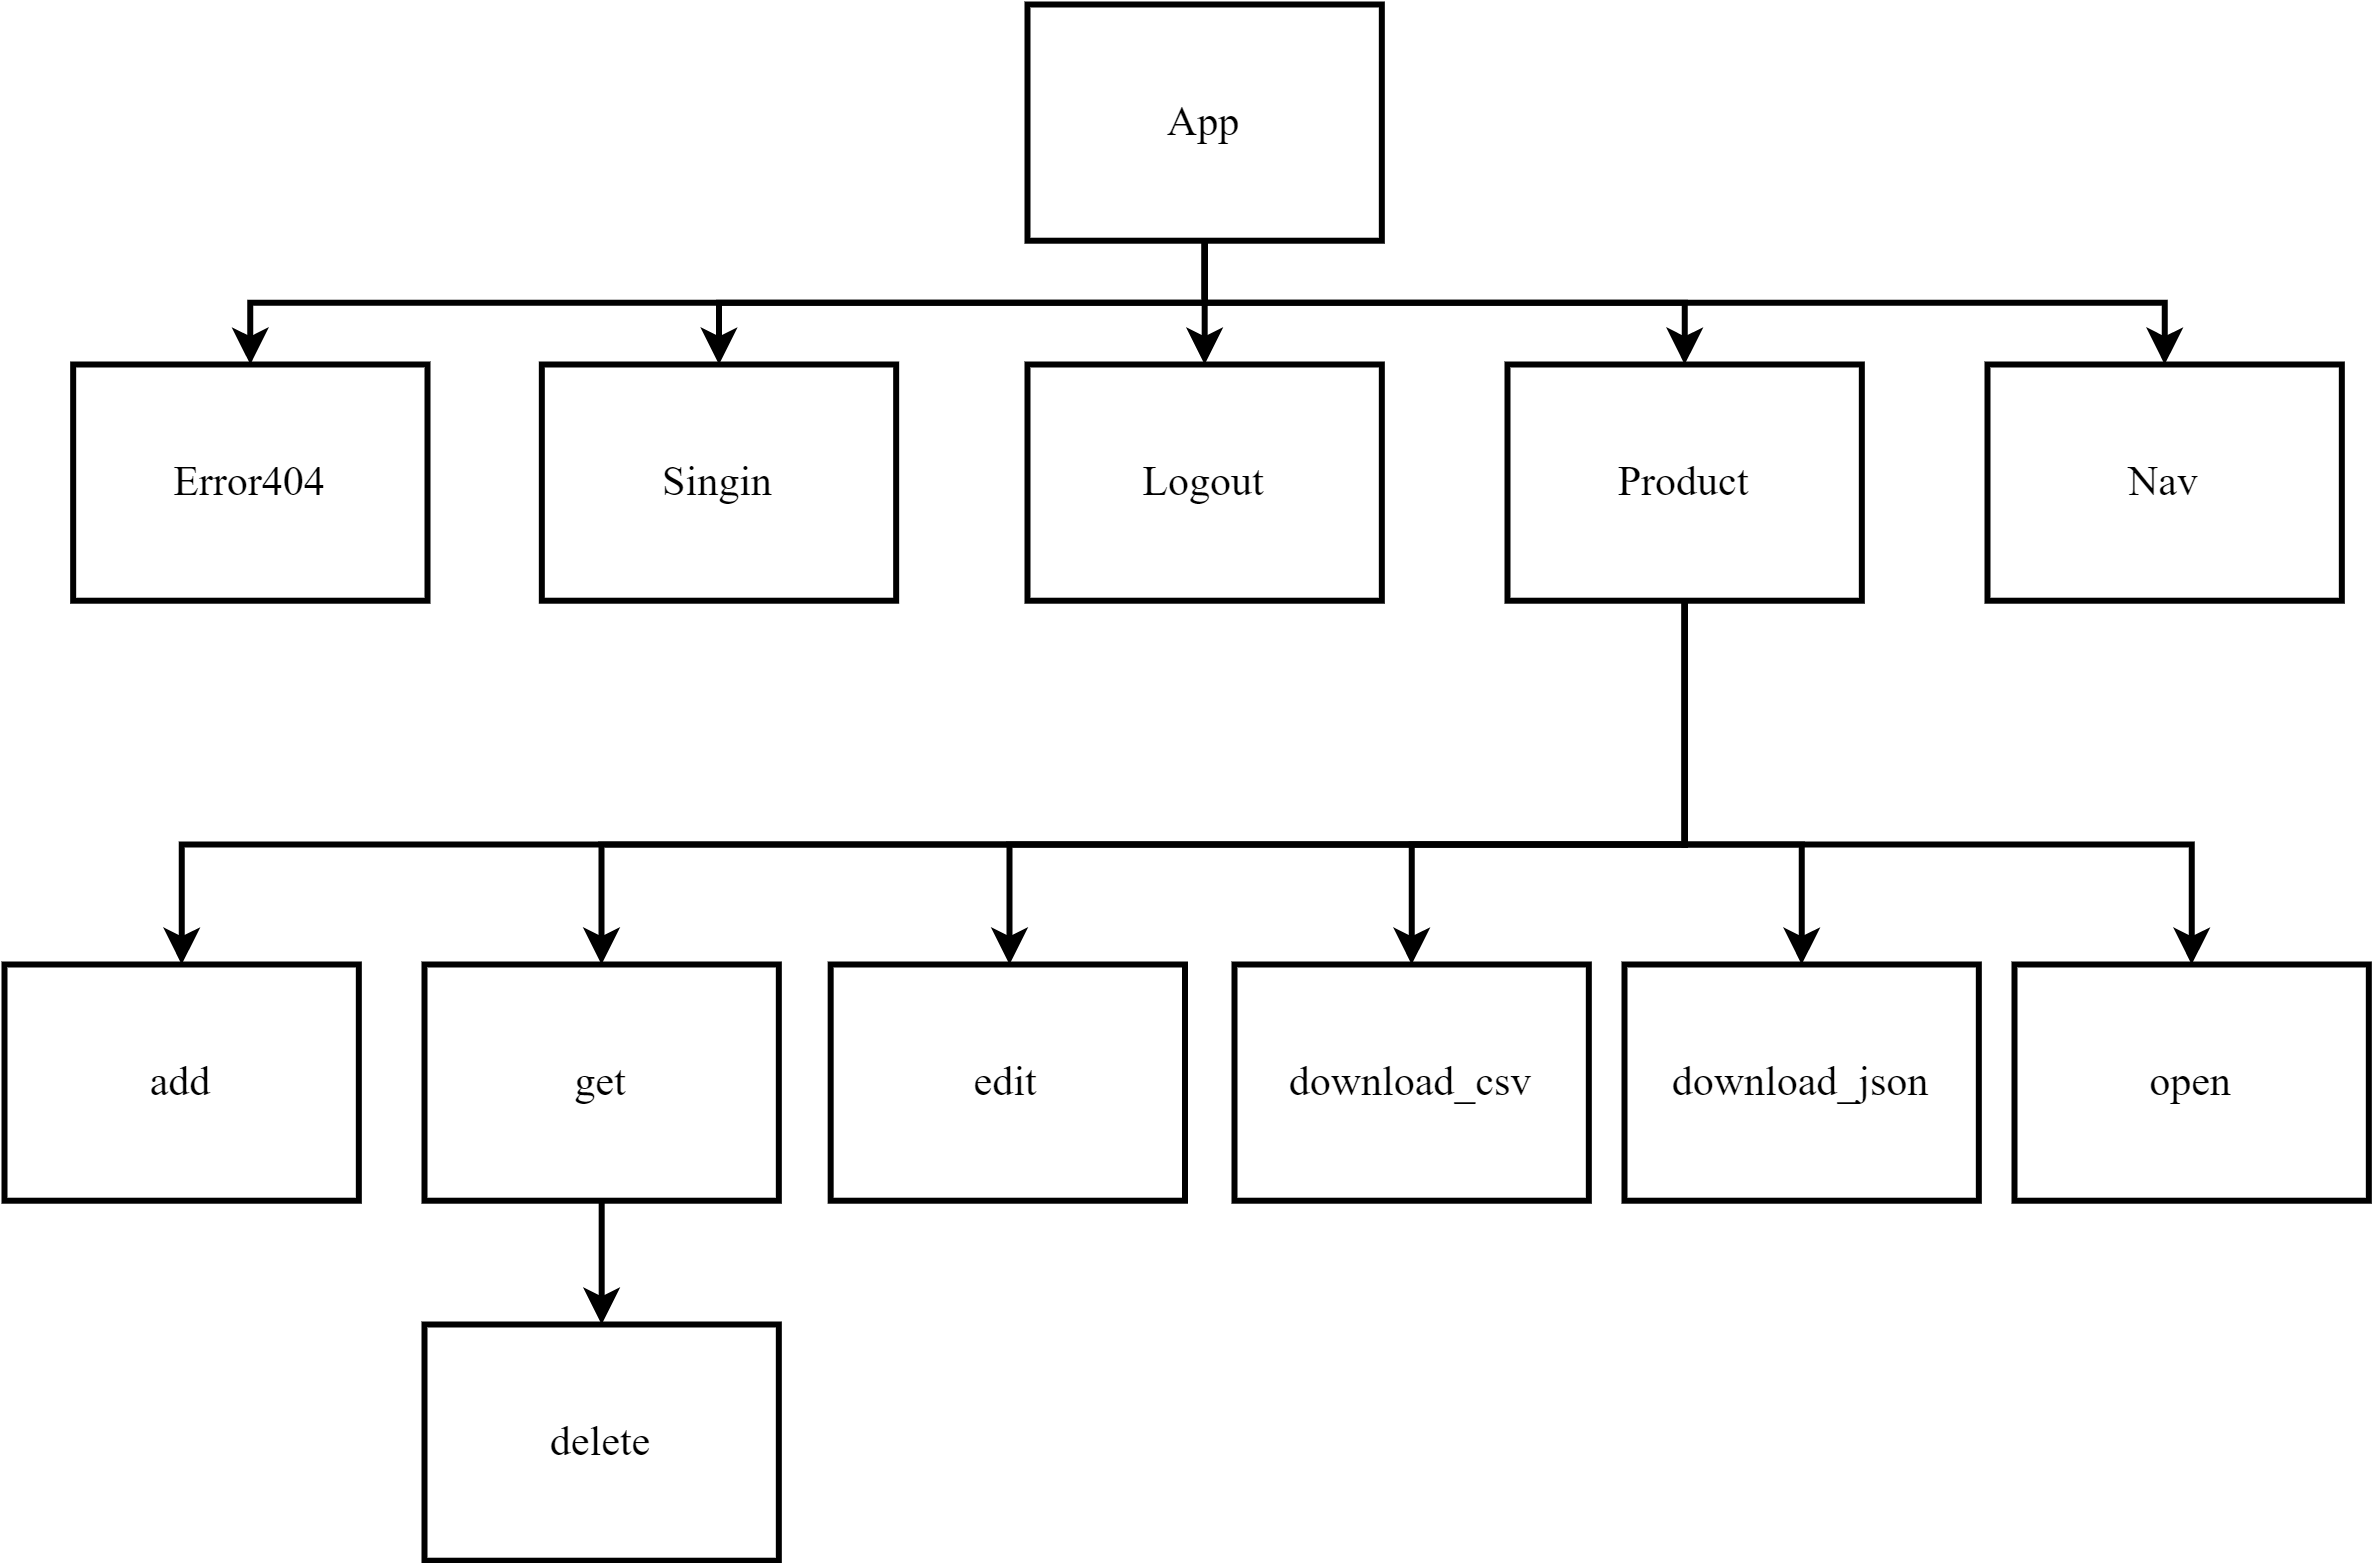
\includegraphics[width=12.5cm]
        {_assets/gpi_frontend_modules.png}
    \caption{Модули и подмодули для frontend}
    \label{fig:gpi_frontend_modules}
\end{figure}

\newpage

\subsubsection*{Иерархия модулей и подмодулей разрабатываемой программы для backend}

Информационная система включает в себя следующие модули на backend:

\begin{itemize}
    \item модуль авторизации;
    \item модуль добавления элементов в базу данных;
    \item модуль вывода элементов сортированных, инвертированных или по ID;
    \item модуль редактирования элемента по ID;
    \item модуль удаления элемента по ID.
\end{itemize}

Схема backend модулей изображена на
\textbf{рис. \ref{fig:gpi_backend_modules} (стр. \pageref{fig:gpi_backend_modules})}.

\begin{figure}[!htp]
    \centering
    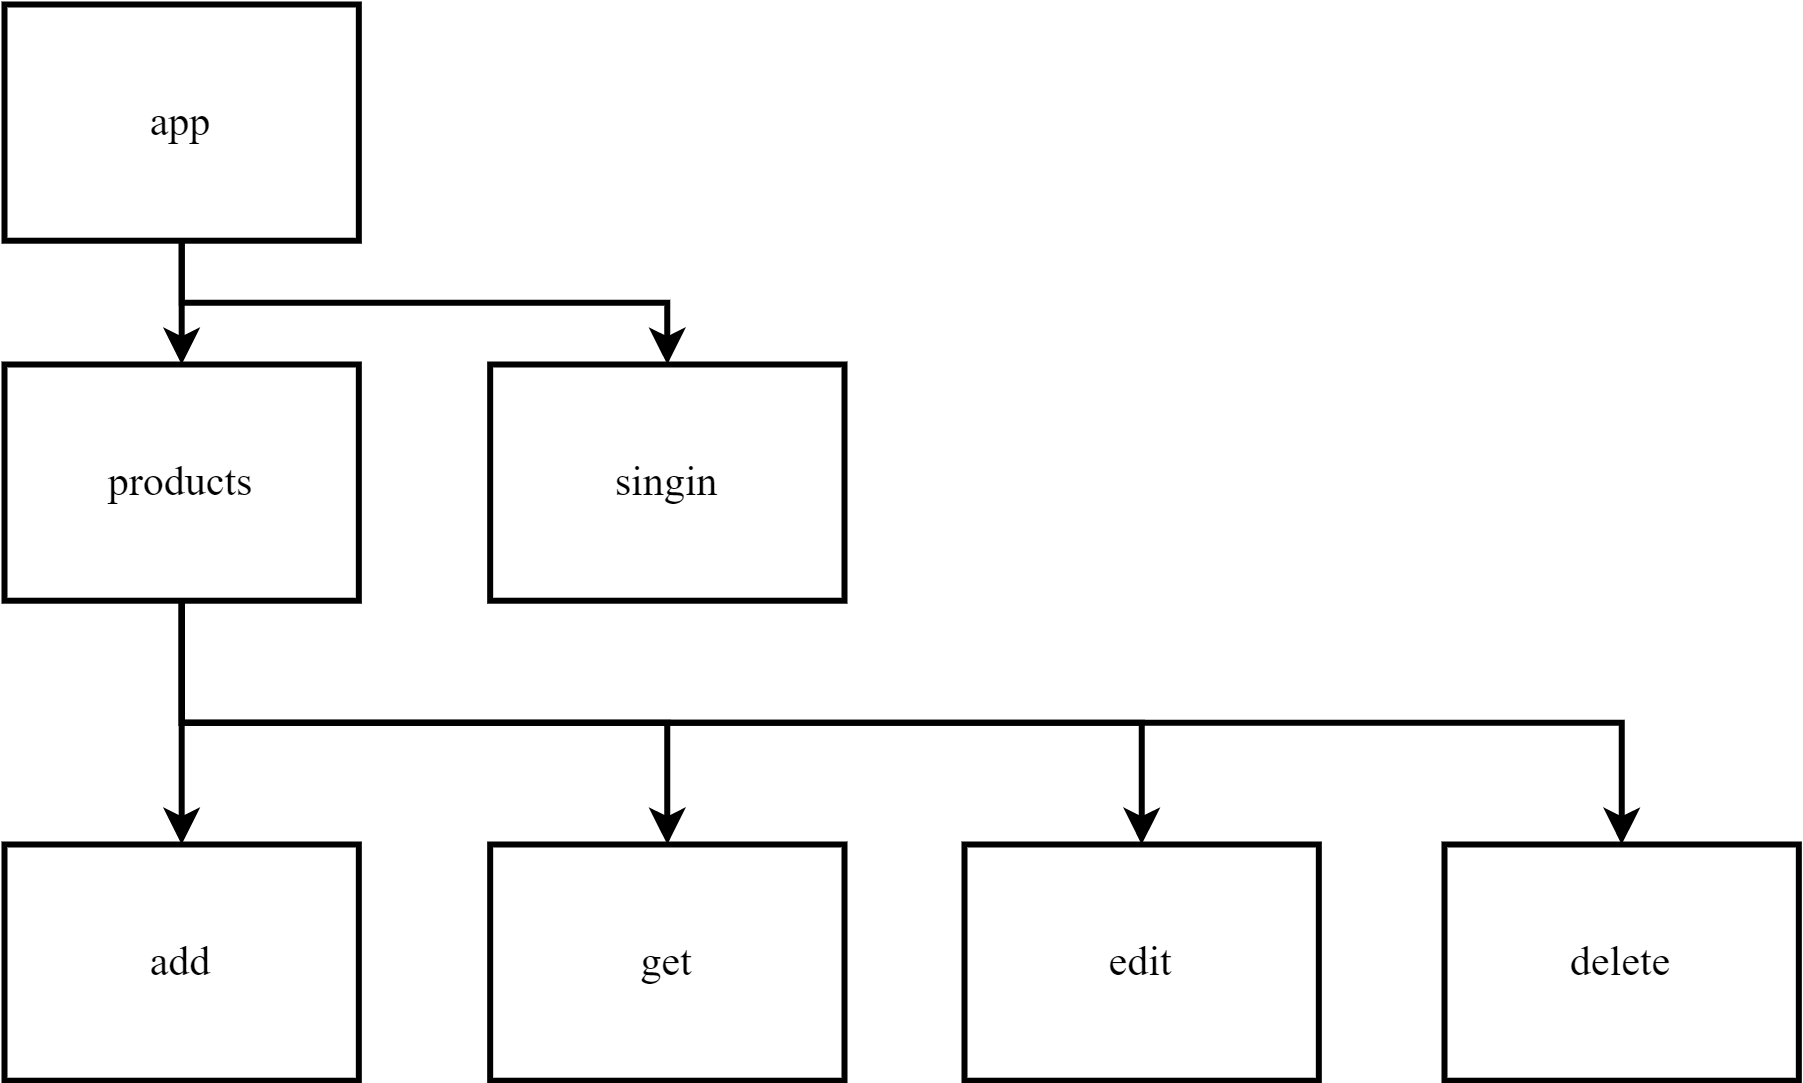
\includegraphics[width=16cm]
        {_assets/gpi_backend_modules.png}
    \caption{Модули и подмодули для backend}
    \label{fig:gpi_backend_modules}
\end{figure}

\newpage
        % Постановка задачи
\end{document}
